%\documentclass[journal]{IEEEtran}
\documentclass[letterpaper,10pt,conference]{ieeeconf}

\IEEEoverridecommandlockouts                              % This command is only
                                                          % needed if you want to
                                                          % use the \thanks command
\overrideIEEEmargins
% See the \addtolength command later in the file to balance the column lengths
% on the last page of the document

\usepackage{amsmath,amssymb}
\usepackage{graphicx}                    % For pdf, bitmapped graphics files
\usepackage[usenames,dvipsnames]{xcolor} % For font in color
\usepackage{eurosym}                     % For writing sybmol for euro
\usepackage{siunitx}                     % For writing SI units
%\usepackage{subfigure}                   % For subfigures
%\usepackage{multirow}                    % Span table cells on multiple rows
%\usepackage{balance}                     % For ballancing the last page

\usepackage[]{units}
\usepackage{comment}
% custom commands
\newcommand{\red}[1]{\textcolor{red}{#1}}  % we use red color for comments

%\author{Nikolce Murgovski, Gabriel Rodrigues de Campos, Jonas Sj\"oberg
%\thanks{The authors are with the Department of Signals and Systems, Chalmers University of Technology, Sweden. {\tt \{nikolce.murgovski, gabriel.campos, jonas.sjoberg\}@chalmers.se.}}%
%\thanks{G. R. Campos is also with the DEIB, Politecnico di Milano, Italy. {\tt gabriel.rodriguesdecampos@polimi.it}}%
%\thanks{The research leading to these results was supported by the grant AD14VARI02 - Progetto ERC BETTER CARS - Sottomisura B, the S2, SAFER, and by the European Commission Seventh Framework Programme under the project AdaptIVe, grant agreement number 610428.}% <-this % stops a space
%}
\author{Markus Carlander, Niklas Lidander, Lea Riegger, Nikolce Murgovski, Jonas Sj\"oberg}
%\thanks{The authors are with the Department of Signals and Systems, Chalmers University of Technology, Sweden. {\tt \{nikolce.murgovski, gabriel.campos, jonas.sjoberg\}@chalmers.se.}}%
%\thanks{G. R. Campos is also with the DEIB, Politecnico di Milano, Italy. {\tt gabriel.rodriguesdecampos@polimi.it}}%
%\thanks{The research leading to these results was supported by the grant AD14VARI02 - Progetto ERC BETTER CARS - Sottomisura B, the S2, SAFER, and by the European Commission Seventh Framework Programme under the project AdaptIVe, grant agreement number 610428.}% <-this % stops a space
%}

\newlength \figwidth
\setlength \figwidth {\columnwidth}


\graphicspath{{figures/}}

\begin{document}
\title{Design and simulation of a centralized MPC for autonomous intersection crossing}

\maketitle
\thispagestyle{empty}
\pagestyle{empty}

%%%%%%%%%%%%%%%%%%%%%%%%%%%%%%%%%%%%%%%%%%%%
\begin{abstract}
This paper proposes a method for a safe and autonomous intersection crossing. A centralized system controls autonomous vehicles within a certain surrounding of the intersection and generates optimized trajectories for all vehicles in this area. By formulating a convex quadratic optimization problem in space domain with respect to collision avoidance constraints, a model predictive controller is designed. To validate the controller for a more advanced vehicle model, a complete simulation environment for virtual test driving is generated by combining CarMaker with Matlab/Simulink. A case study shows the effectiveness of the proposed method.
\end{abstract}

\IEEEpeerreviewmaketitle

\section{Introduction}%from the planning report, we have to change that a bit

Around the world, traffic accidents that are related to intersections occur all too often. Compiled statistic from several European Countries shows that 43$\%$ of all road injury accidents can be related to intersections \cite{molinero}. Statistic conducted in the USA indicates similar numbers \cite{nhtsa}. The actual number of related traffic accidents in Sweden is slightly less in total. Of all reported accidents in the year 2014 in Sweden, 24$\%$ are intersection related. Of those, 91 $\%$ led to severe person injuries \cite{sverige}. As the statistics show, intersections lead to high risk for accidents. Even though the most dangerous intersections are regulated by traffic lights, signs and road-markings, accidents occur still very frequently. Higher safety in intersection crossing comes at a price in today's society since it limits the traffic flow. This causes bottlenecks in the traffic rhythm which not only wastes a lot of time for travelers but also leads to environment pollution caused by unnecessary accelerations and decelerations.\\ \indent
Today's vehicles are trending to become more and more autonomous. Exclusive benefits as adaptive cruise control, automatic lane change maneuvers, parking assistance are available on the market today. Statistic from USA shows that about 96$\%$ of all intersection related accidents are attributed to drivers \cite{nhtsa}. If intersections would be controlled by an autonomous cooperative intersection algorithm that can optimize the crossing sequence for all nearby vehicles, the intersection should be more safe since no human factor would cause any accident. The intersection should also be more efficient in both terms, time and energy consumption, since the algorithm would decide in which order the vehicles should pass for maximum efficiency. Aspects as minimizing deceleration, respectively acceleration, as well as reducing the total time for the intersection crossing will be taking into account for computing the optimal crossing sequence. It would also be possible to set different priority orders for different types of vehicles, for example according to their fuel consumption. Emergency vehicles could also be given precedence to enter the intersection on call-out.\\ \indent
In this paper, a Model Predictive Controller (MPC) is designed for a centralized system which takes control over autonomous vehicles within a certain surrounding of the intersection. The vehicles are assumed to drive fully autonomous. Due to the trend to self-driving vehicles, a lot of research in this area has been done. Among other recent work some have already exploited the idea of using MPC with different approaches \cite{eleven}, \cite{twelve},\cite{thirteen}, \cite{fourteen}, \cite{fifteen}. In \cite{thirteen} for example, the solution is approximated by a centralized, finite time optimal control problem. In \cite{fourteen}, a decentralized approach based on sub-optimal
decision-making heuristics is used. The general optimization algorithm for intersection crossing in this paper is based on the approach \cite{nikolce} where the problem is formulated as a convex optimization problem for each possible crossing sequences. In each time step, the designed MPC generates optimized trajectories for all vehicles in the controlled area, such that a cost function is minimized and several constraints are fulfilled. The cars may differ in speed, acceleration and their braking capabilities. The controller is tested for a case study using the simulation tool CarMaker, which provides complex vehicle models, in combination with Matlab/Simulink. 

The paper has therefore two main subjects: 
\begin{itemize}
\setlength\itemsep{0.3em}
\item Designing a Centralized MPC Controller,
\item Implementation \& Simulation Using CarMaker.
\end{itemize}
Even though the design of the MPC controller is a highlighted area, the focus of this article will be on the implementation and simulation using CarMaker.\\ \indent The paper is organized as follows: Section II gives an overview of the convex problem formulation in space domain. In Section III an MPC is designed. Section IV describes the simulation procedure. A simulation environment, constructed in CarMaker, and the MPC, designed in Matlab/Simulink, is combined. Section V shows a case study that tests if the controller is efficient in the simulation environment. Section VI closes the paper with final conclusions.

\section{Problem Formulation} 
This section presents a way of formulating the autonomous intersection crossing as a convex optimization problem. 
\subsection{Assumptions}
The vehicles entering the intersection have a predefined path and are assumed to follow their path. Considering $N_v$ autonomous vehicles in a surrounding of an intersection, it is assumed that for each vehicle $i$, the acceleration along the path can be varied. The presented intersection crossing scenario is limited to one vehicle per lane which means that the scenario where vehicles are following each other on the same lane is not studied. Nevertheless, the controller is designed in a way that an adaption to enable this is possible.
\subsection{Convex problem statement}
In the optimization problem, the vehicle dynamics are simplified to a point mass model. To formulate the optimization problem in a convex form, it is sampled in space, rather than time.
With the spatial coordinate $p$, the linear state space model
\begin{align}\label{statesp}
\begin{split}
\kappa_i'(p)&=\underbrace{\begin{pmatrix}
0& 1\\
0& 0
\end{pmatrix}}_{\hat{A}}\kappa_i(p) + \underbrace{\begin{pmatrix}
0\\
1\end{pmatrix}}_Bu_i(p)\\
y_i(p) &= \underbrace{\begin{pmatrix}
0 & 1
\end{pmatrix}}_C\kappa_i(p)
\end{split}
\end{align}
is used to model each vehicle $i$, where $\kappa_i=\begin{pmatrix}t_i(p)& z_i(p)\end{pmatrix}^T$ is the state vector and $\kappa_i'=d\kappa/dp$ is the derivative with respect to distance. The lethargy $z_i(p)=1/v_i(p)$ indicates the slowness of the system. Input $u_i(p)$ is the spatial derivative of $z_i(p)$. 
According to \cite{nikolce}, the convex problem can be formulated as following:
\subsubsection{Cost function}
The cost function for each car $i$ can be summed up to the total cost function 
\begin{align}
\min_{u_i(p)} \sum_{i=1}^{N_v}
J_i(\kappa_i(p), u_i(p), u_i'(p), \kappa_i(p_{if}))\, \label{costspace}
\end{align}
where $p_{if}$ is the final position.
Using weighting factors $w_{ij}$, the convex cost function for each vehicle $i$ can be chosen as
\begin{equation}\label{eq:costfnc}
J_i(z_i(p)) \approx J_{i1}+J_{i2}+J_{i3}.
\end{equation}
The first term
\begin{subequations}
\begin{equation}
J_{i1}(z_i(p))\approx w_{i1}\bar{v}_{ir}^3 \int_0^{p_{if}}(z_i(p)-\frac{1}{v_{ir}(p)})^2
\label{cost1}
\end{equation}
penalizes the deviation from the reference velocity. 
The mean of the reference velocity $v_{ir}(p)$ for each car $i$ is $\bar{v}_{ir}$. The term $J_{i2}+J_{i3}$ with
\begin{align}
J_{i2}(z_i(p)) \approx w_{i2}\bar{v}^5_{ir}
\int_0^{p_{if}}u^2_i(p),\\
J_{i3}(z_i(p)) \approx w_{i3}\bar{v}_{ir}^7\int_0^{p_{if}}u_i'^2(p)
\end{align}
\end{subequations}
penalizes high longitudinal acceleration and jerk to guarantee a comfortable drive and limit actuator usage.
\subsubsection{Constraints}
The constraints are the state space model, limitations for the state vector $\kappa_i$ and the input $u_i$ as well as initial and final state constraints:
\begin{subequations}\label{eq:constraints}
\begin{align}
\kappa_i'(p) &= A\kappa_i(p) + Bu_i(p)\label{eq:spm}\\
\kappa_i(p) &\in [\kappa_{imin}(p), \kappa_{imax}(p)]\label{eq:vlim}\\
%ignore u constraint first????
u_i(p) &\in [u_{imin}(p, z_i(p)), u_{imax}(p, z_i(p))]\label{eq:ulim}\\
\kappa_{i}(0)&=\kappa_{i0} = \begin{pmatrix}0& 1/v_{i0}\end{pmatrix}^T\\
\kappa_{i}(p_{if})&=\kappa_{if} = \begin{pmatrix}\mathrm{free}& 1/v_{if} \end{pmatrix}^T\label{eq:free},
\end{align}
where the limits of \eqref{eq:ulim} are linear functions of $z_i$. To avoid collisions, a final constraint is needed, which guarantees, that a car can only enter the intersection, when the previous car has left the intersection: 
\begin{align}
\begin{split}
t_k(H_k) \leq t_l(L_l),\; k&=\Omega_{m,n},\; l=\Omega_{m,n+1}\label{eq:col},\\
n&=1,\dots, N_v-1, 
\end{split}
\end{align}
\end{subequations}
where $k$ and $l$ are indices of the vehicles in a given crossing sequence $m$ of the permutation matrix $\Omega$, which contains all possible crossing sequences. Position $H_k$ is the point when vehicle $k$ exits the critical set. Position $L_l$ is the entering point for vehicle $l$.
For a given crossing sequence, the optimization problem is a convex quadratic program.\\ \indent
More detailed explanations about the convex modeling of the problem can be found in \cite{nikolce}.
\section{MPC Design}
\subsection{Discrete state space model}
In order to implement the controller in Matlab, a discrete version of the model \eqref{statesp} with a sampling interval of $\unit[1]{m}$  is derived. The result is the following discrete state space representation:
\begin{align}
\label{eq:model}
\begin{split}
\kappa_i(p+1) &= \underbrace{\begin{pmatrix}
1 & 1  \\
0 & 1 
\end{pmatrix}}_A
\kappa_i(p)
+
\underbrace{\begin{pmatrix}
0 \\
1
\end{pmatrix}}_Bu_i(p)\\
y_i(p) &= \underbrace{\begin{pmatrix}
0 & 1
\end{pmatrix}}_C\kappa_i(p).
\end{split}
\end{align}
%where $\kappa_i(p) = \begin{pmatrix}
%t_i(p) \\
%z_i(p)
%\end{pmatrix}$ and $u = z'_i$ for each vehicle %$i$ respectively.
\subsection{Extended cost function}
To avoid the risk of infeasible solutions for the minimization problem when several cars are very close to the critical region, or worse, violate the constraint that restricts more than one vehicle to be inside the critical region at the same time, the optimization problem is extended.\\ \indent
An extra slack variable $s_j$ for each consecutive vehicle pair inside the control region is added. The variable $s_j$ expresses the time difference between the first vehicle of the pair leaving the intersection and the second vehicle entering the intersection. By predefining a suitable time difference $\Delta t$, the cost function \eqref{costspace} can be extended by 
\begin{subequations}\label{slackall}
\begin{align}\label{eq:smin}
\min_{s_j}  \sum_{j=1}  &w_{j}\max (0,\Delta t -  s_j)^2 
\end{align}
and the constraints \eqref{eq:spm}-\eqref{eq:free} can be extended by
\begin{align}
\label{eq:saeq}
& s_j = t_l(L_l) - t_k(H_k)\\
& s_j \geq 0.\label{eq:sain}
\end{align} 
\end{subequations}
The maximization in \eqref{eq:smin} is a convex function that minimizes the difference between the slack variable $s_j$ and $\Delta t$ for vehicle pairs where $t_l(L_l)-t_k(H_k) < \Delta t$. Vehicle pairs in which the vehicles are far apart are not forced to have a predefined time difference in the crossing.
The constraints \eqref{eq:saeq} and \eqref{eq:sain} let the slack variable fulfill the description and keep the original constraint \eqref{eq:col} that only one car can be inside the critical set.\\ \indent
Further can \eqref{eq:smin} be rewritten as
\begin{subequations}\label{qdef}
\begin{align}\label{eq:qmin}
\min_{s_j}  \sum_{j=1}  &w_{j} q_j^2 
\end{align}
and the maximization can be expressed by two linear constraints:
\begin{align}
& q_j \geq \Delta t - s_j\label{eq:geq1}\\ 
& q_j \geq 0.\label{eq:qgeq2}
\end{align} 
\end{subequations}
\subsection{Transformation to a standard quadratic problem}
In order to solve the minimization problem in \eqref{costspace} and \eqref{eq:constraints} with the quadratic program (QP) solver \emph{quadprog} in Matlab, the formulation must first be transformed into the standard form 
\begin{subequations} \label{stform}
\begin{align}\label{eq:quad}
\min_{x}& \frac{1}{2}x^THx+f^Tx\\
\text{subject to } 
&A_{eq}x =b_{eq},\label{eq:aeq}\\
&A_{in}x \leq b_{in}.\label{eq:ain}
\end{align}
\end{subequations}
where $x$ is the wanted vector that minimizes the cost function, $H$ the hessian matrix and $f$ the remaining terms that are not in quadratic form. The constraints in \eqref{eq:spm}-\eqref{eq:col} also need to be transformed such that they fit the new constraint formulation in \eqref{eq:aeq}-\eqref{eq:ain}.
\subsubsection{Cost function}
The cost function \eqref{eq:costfnc} is transformed in a quadratic form for the MPC by writing the $x=\begin{pmatrix}x_1&\dots&x_{N_v}  \end{pmatrix}^T$ vector in \eqref{eq:quad} as
\begin{equation}
x_i=\begin{pmatrix}
\kappa_i(p+1)\\\vdots\\ \kappa_i(p+N)\\ u_i(p) \\ \vdots \\ u_i(p+N-1)\\ u_i'(p)\\ \vdots \\ u_i'(p+N-1) 
\end{pmatrix}
\end{equation}
for each vehicle $i$ in the control region. The vector $x_i$ involves the states, the control input and the derivative of the control input. The prediction and control horizon are both equal to N. The Hessian matrix $H_i$ for each vehicle $i$ results in
\begin{equation}\label{eq:hessian}
H_i = 2
\begin{pmatrix}
    Q_{i1} & 0 & 0 \\
    0 & Q_{i1} & 0 \\
    0 & 0 & Q_{i1} \\
\end{pmatrix},
\end{equation}
where the matrices $Q_{i1}, Q_{i2}$ and $Q_{i3}$ are equal to
\begin{subequations}
\begin{align}
Q_{i1} &= w_{i1}\bar{v}_{ir}^3 C^TC I_N, \\ 
Q_{i2} &=  w_{i2}\bar{v}_{ir}^5I_N ,\\
Q_{i3} &= w_{i3}\bar{v}_{ir}^7I_N,
\end{align}
\end{subequations}
where $I_N$ is the identity matrix with $N$ rows.
The $f_i$ vector containing the remaining non-quadratic terms for each vehicle $i$ is
\begin{equation}
f_i^T = -2w_{i1}\bar{v}_{ir}^3\frac{1}{v_{ir}(p)}C
\begin{pmatrix}
1 & \hdots & 1 & 0 & \hdots & 0
\end{pmatrix}\label{eq:fvec}.
\end{equation}
%
%
\begin{comment}
According to \eqref{eq:smin}, the Hessian matrix $H_{sj}$ for each slack variable $s_j$ can be formulated in the following way:
\begin{equation}
\label{eq:Hs}
H_{sj} =
2w_j.
\end{equation}
The vector $f_{sj}$ contains the remaining non-quadratic terms of \eqref{eq:smin}:
\begin{equation}
\label{eq:fs}
f_{sj}^T = -2w_j\Delta t.
\end{equation}
The resulting total quadratic cost function is
\begin{equation}
\min_{x_i, s_j} \sum_{i} \frac{1}{2}x_i^TH_ix_i+f_i^Tx_i+\sum_{j} \frac{1}{2}s_j^TH_{sj}s_j+f_{sj}^Ts_j.\\
\end{equation}
\end{comment}
%
%
According to \eqref{eq:qmin}, the Hessian matrix $H_{q_j}$ for each variable $q_j$ can be formulated in the following way:
\begin{equation}
\label{eq:Hs}
H_{q_j} =
2w_j.
\end{equation}
The resulting total quadratic cost function is
\begin{equation}\label{cost12}
\min_{x_i, s_j, q_j} \sum_{i} \frac{1}{2}x_i^TH_ix_i+f_i^Tx_i+\sum_{j} \frac{1}{2}q_j^TH_{q_j}q_j.\\
\end{equation}
%missing: definitions of w, v_ir etc.
\subsubsection{Constraints}
%The state constraint of the model in \eqref{eq:spm} can be written in the new equality constraint formulation \eqref{eq:aeq} as
The state constraint of the model described in \eqref{eq:spm} has to be reformulated in a matrix form as shown in \eqref{eq:aeq} with the discrete model described in \eqref{eq:model}. In addition, two more equality constraints can be added on $u_i(p)$ and $u'_i(p)$ to avoid a random initialization point. The slack variables need also to be added into the matrices for all consecutive vehicle pairs that are inside the control region. This results in 
\begin{align}\label{eq1car}
        \begin{cases}
            A\kappa_i(p+n)-\kappa_i(p+n+1) - Bu_i(p+n) = 0\\
            u_i(p) = u_i(p-1)\\
            u'_i(p) = u'_i(p-1)
        \end{cases}
\end{align}
with $n=1,\dots,N$ and 
\begin{align}\label{eq1car2}
    t_l(L_l) - t_k(H_k) -s_j = 0
\end{align}
for the slack variable.\\ \indent
\begin{comment}
\begin{equation}
A_{eq} = \begin{pmatrix}
A_{eq1} & A_{eq2} & A_{eq3} 
\end{pmatrix},\;
    b_{eq} = \begin{pmatrix}
    -A\kappa_{ref} \\
    0 \\
    \vdots \\
    0
    \end{pmatrix}   
\end{equation}
where $A_{eq1}$, $A_{eq2}$ and $A_{eq3}$ are written as follows
\begin{equation*}
\begin{aligned}
    A_{eq1} =& \begin{pmatrix}
    -I_2 & 0 & 0 & 0 \\
    A & \ddots & 0 & 0\\
    0 & \ddots & \ddots & 0 \\
    0 & 0 & A & -I_2
    \end{pmatrix},  \\
    A_{eq2} =& \begin{pmatrix}
    B & 0 & 0 & 0 \\
    0 & \ddots & 0 & 0\\
    0 & 0 & \ddots & 0 \\
    0 & 0 & 0 & B
    \end{pmatrix} \,\,  and\\
    A_{eq3} =& \begin{pmatrix}
    0 & 0 & 0 & 0 \\
    0 & \ddots & 0 & 0\\
    0 & 0 & \ddots & 0 \\
    0 & 0 & 0 & 0
    \end{pmatrix}.  
\end{aligned}
\end{equation*}
\end{comment}
Furthermore, the constraints \eqref{eq:vlim}-\eqref{eq:ulim} limiting the state variables and the acceleration as well as the collision avoidance constraint \eqref{eq:col} can be written into new inequality constraints \eqref{eq:ain}. The two constraints \eqref{eq:vlim}-\eqref{eq:ulim} have to be split up into two constraints in order to be implemented in a matrix form. In addition to \eqref{eq:vlim} the acceleration constraints are linearized at the current speed instead of the reference speed as done in \cite{nikolce}. This removes possible linearization errors by re-optimization. The inequality constraints for the MPC are
\begin{align}\label{ineq}
        \begin{cases}
            z_i(p+n) \leq \frac{1}{v_{min}} \\
            -z_i(p+n) \leq -\frac{1}{v_{max}}  \\
            u_i(p+n-1) + \frac{3a_{min}}{v_{i}(p)^2}z_i(p+n-1) \leq \frac{2a_{min}}{v_{i}(p)^3} \\
            -u_i(p+n-1) - \frac{3a_{max}}{v_{i}(p)^2}z_i(p+n-1) \leq -\frac{2a_{max}}{v_{i}(p)^3} \\
        \end{cases}
\end{align}
for each car $i$ and
\begin{align}\label{ineq2}
        \begin{cases}
            - s_j \leq 0\\
            - s_j - q_j \leq - \Delta t\\
            -q_j \leq 0
        \end{cases}    
\end{align}
for each consecutive vehicle pair in the control region.\\ \indent
In order to control $N_v$ vehicles, the QP formulation \eqref{stform} needs to be extended. The new $x$ vector and Hessian matrix for $N_v$ cars are then according to \eqref{cost12}
\begin{comment}
\begin{equation*}
x=\begin{pmatrix}
x_{1} \hdots  x_{N_v} \ s_1 \hdots s_{N_v-1}
%x_{1}\\ \vdots \\ x_{Nv} \\ s_1 \\ \vdots \\ s_{Nv-1}
\end{pmatrix} ^T
\end{equation*}
\begin{equation*}
H = \begin{pmatrix}
    H_1 & 0 & 0 & 0 & 0 & 0\\
    0 & \ddots & 0 & 0 & 0 & 0\\
    0 & 0 & H_{N_v} & 0 & 0 & 0\\
    0 & 0 & 0 & H_{s_1} & 0 & 0\\
    0 & 0 & 0 & 0 & \ddots & 0\\
    0 & 0 & 0 & 0 & 0 & H_{s_{N_v-1}}
\end{pmatrix}
\end{equation*}
\end{comment}
%\begin{equation*}
%x=\begin{pmatrix}
%x_{1} \hdots  x_{Nv} \ s_1 \hdots s_{Nv-1}
%x_{1}\\ \vdots \\ x_{Nv} \\ s_1 \\ \vdots \\ s_{Nv-1}
%\end{pmatrix} \ H = \begin{pmatrix}
%    H_1 & 0 & 0 & 0 & 0 & 0\\
%    0 & \ddots & 0 & 0 & 0 & 0\\
%    0 & 0 & H_{Nv} & 0 & 0 & 0\\
%    0 & 0 & 0 & H_{s_1} & 0 & 0\\
%    0 & 0 & 0 & 0 & \ddots & 0\\
%    0 & 0 & 0 & 0 & 0 & H_{s_{Nv-1}}
%\end{pmatrix}
%\end{equation*}
%\begin{align}
%x &=\begin{pmatrix}
%x_1 & \hdots & x_{N_v} & q_1 & \hdots & q_{N_v-1}
%\end{pmatrix}^T,\\
%H &= diag(H_1\; \dots\; H_{N_v}\; H_{q_1} \;\dots\; H_{q_{N_v-1}}),
%\end{align}
\begin{align}
x &=\begin{pmatrix}
x_{1:N_v}^T & s_{1:N_v-1} & q_{1:N_v-1}
\end{pmatrix}^T,\label{xvec}\\
H &= diag\begin{pmatrix}H_{1:N_v}&0 \; \dots \; 0 & H_{q_1:q_{N_v-1}}\end{pmatrix},
\end{align}
where $q_j$ and $s_j$ are the variables defined in \eqref{slackall} and \eqref{qdef}. The $f$ vector is changed to the following
%\begin{equation}
%f^T = 
%\begin{pmatrix}
%    f_1 & \hdots & f_{N_v} & 0 & \hdots & 0
%\end{pmatrix}
%\end{equation}
\begin{equation}
f^T = 
\begin{pmatrix}
f^T_{1:N_v} & 0 \; \dots \; 0
\end{pmatrix}.
\end{equation}
To control all $N_v$ cars, the constraints also change in the same manner as the Hessian matrix.
Using the $x$ vector \eqref{xvec}, the equality constraints \eqref{eq1car} and \eqref{eq1car2} for all $i=1,\dots, N_v$ vehicles and $j=1,\dots, N_v-1$ slack variables can be written as 
\begin{align}
    A_{eq,i}x&=b_{eq,i}, \\
    A_{eq,sj}x&=b_{eq,sj}
\end{align}
and combined to the standard form \eqref{eq:aeq} such that
\begin{align}
A_{eq}^T&=
\begin{pmatrix}
    A_{eq,1:N_v}^T & A_{eq,s1:sN_v-1}^T
    \end{pmatrix},\\
    b_{eq}^T&=\begin{pmatrix}
    b_{eq,1:N_v}^T & b_{eq,s1:sN_v-1}^T
    \end{pmatrix}.
\end{align}
Analogous, the inequality constraints \eqref{ineq} and \eqref{ineq2} can be transformed to
\begin{align}
    A_{in,i}x&=b_{in,i}, \\
    A_{in,sj}x&=b_{in,sj}.
\end{align}
Taking all vehicles and slack variables into account, the result can be written in the desired form \eqref{eq:ain} with
\begin{align}
A_{in}^T&=
\begin{pmatrix}
    A_{in,1:N_v}^T & A_{in,s1:sN_v-1}^T
    \end{pmatrix},\\
    b_{in}^T&=\begin{pmatrix}
    b_{in,1:N_v}^T & b_{in,s1:sN_v-1}^T
    \end{pmatrix}.
\end{align}
\begin{comment}
The constraints also change in the same manner as the Hessian matrix.
The equality constraints are set as
\begin{align}
        \begin{cases}
            A\kappa_{1:N_v}(p+n)-\kappa_{1:N_v}(p+n+1) - Bu_{1:N_v}(p+n) = 0\\
            u_{1:N_v}(p) = u_{1:N_v}(p-1)\\
            u'_{1:N_v}(p) = u'_{1:N_v}(p-1)\\
            t_l(L_l) - t_k(H_k) -s_{1:N_v-1} = 0\\
        \end{cases}
\end{align}
%\begin{align*}
%A_{eq}&=
%\begin{pmatrix}
%    A_{eq1} & 0 & 0 & 0 & 0 & 0 & 0 \;\dots\; 0\\
%    0 & \ddots & 0 & 0 & 0 & 0& 0 \;\dots\; 0\\
%    0 & 0 & A_{eq_{N_v}} & 0 & 0 & 0& 0 \;\dots\; 0\\
%    -t_{k_1} & t_{l_1} & 0 & -s_1 & 0 & 0& 0 \;\dots\; 0 \\
%    0 & \ddots & \ddots & 0 & \ddots& 0 & 0 \;\dots\; 0\\
%    0 & 0 & -t_{k_{N_v-1}} & -t_{l_{N_v-1}} & & -s_{N_v-1} & 0 \;\dots\; 0\\
%\end{pmatrix},\\
%b_{eq}&=\begin{pmatrix}
%b_{eq1}\\ \vdots \\ b_{eq_{Nv}} \\ 0_1 \\ \vdots \\ 0_{Nv-1}
%b_{eq1} \hdots b_{eq_{N_v}} \ 0_1  \hdots  0_{N_v-1}
%\end{pmatrix}^T,
%\end{align*}
where the last $N_v-1$ rows and last $N_v-1$ columns in $A_{eq}$ as well as the last $N_v-1$ rows in $b_{eq}$ are due to the introduction of the slack variables. Similarly, the inequality constraints are formulated as
\begin{equation*}
\begin{aligned}
%A_{in}&= diag( A_{in1}\; \dots\; A_{in_{N_v}}\; -s_1 \;\dots\; -s_{N_v-1}),\\
A_{in}&= ( A_{in_j} A_{in_j})^T,\\
%\begin{pmatrix}
%    A_{in1} & 0 & 0 & 0 & 0 & 0\\
%    0 & \ddots & 0 & 0 & 0 & 0\\
%    0 & 0 & A_{in_{Nv}} & 0 & 0 & 0\\
%    0 & 0 & 0 & -s_1 & 0 & 0\\
%    0 & 0 & 0 & 0 & \ddots & 0\\
%    0 & 0 & 0 & 0 & 0 & -s_{Nv-1}
%\end{pmatrix},
b_{in}&=\begin{pmatrix}
%b_{in1}\\ \vdots \\ b_{in_{Nv}} \\ 0_1 \\ \vdots \\ 0_{Nv-1}
b_{in1} \hdots b_{in_{N_v}} \ 0_1 \hdots 0_{N_v-1}
\end{pmatrix}^T,
\end{aligned}
\end{equation*}
with the last $N_v-1$ rows are due to the slack variables.
%\textit{Note that the definition of the vector $x$ and thus also all other matrices shown in this section may vary depending on the distance to the intersection of each vehicle. For example, when only the first vehicle is within the control region, the vector is $x = x_1$.}
\end{comment}
\subsection{Control area and optimization horizon}
Whether a vehicle is included in the MPC computation depends on its distance to the intersection. The control area of the centralized controller is defined for a certain surrounding of the intersection. Before entering the control area, it is assumed that the car drives with its reference speed. The control area is re-scanned in every time step searching for new arriving or leaving cars. The controller re-optimizes in every time step and takes therefore only the vehicles in the control area into account. The re-optimization is needed because the vehicles do not follow exactly the desired acceleration computed by the controller due to the simplified point mass model for the vehicle dynamics in the controller.\\ \indent
%Another important point is that the acceleration limits in space domain are convexified in \cite{nikolce} by linearizing $z^3_i(p)$ around the reference speed. Re-linearizing around the actual optimal velocity trajectory, as done in \eqref{ineq}, decreases the linearization error. This is another reason for the re-optimization.\\\\ \indent
Since there is no point in controlling the vehicles after they have passed the control radius, the optimization horizon $N$ is not moving along the vehicles as they advance. Instead the horizon is fixed to the end of the control radius. In this way, the optimization horizon is shrinking as the cars are progressing through the control area. This lowers the computation time of the MPC algorithm in each position step of the vehicles in the control area.
\section{Simulation}
\begin{figure*}[]
    \centering
    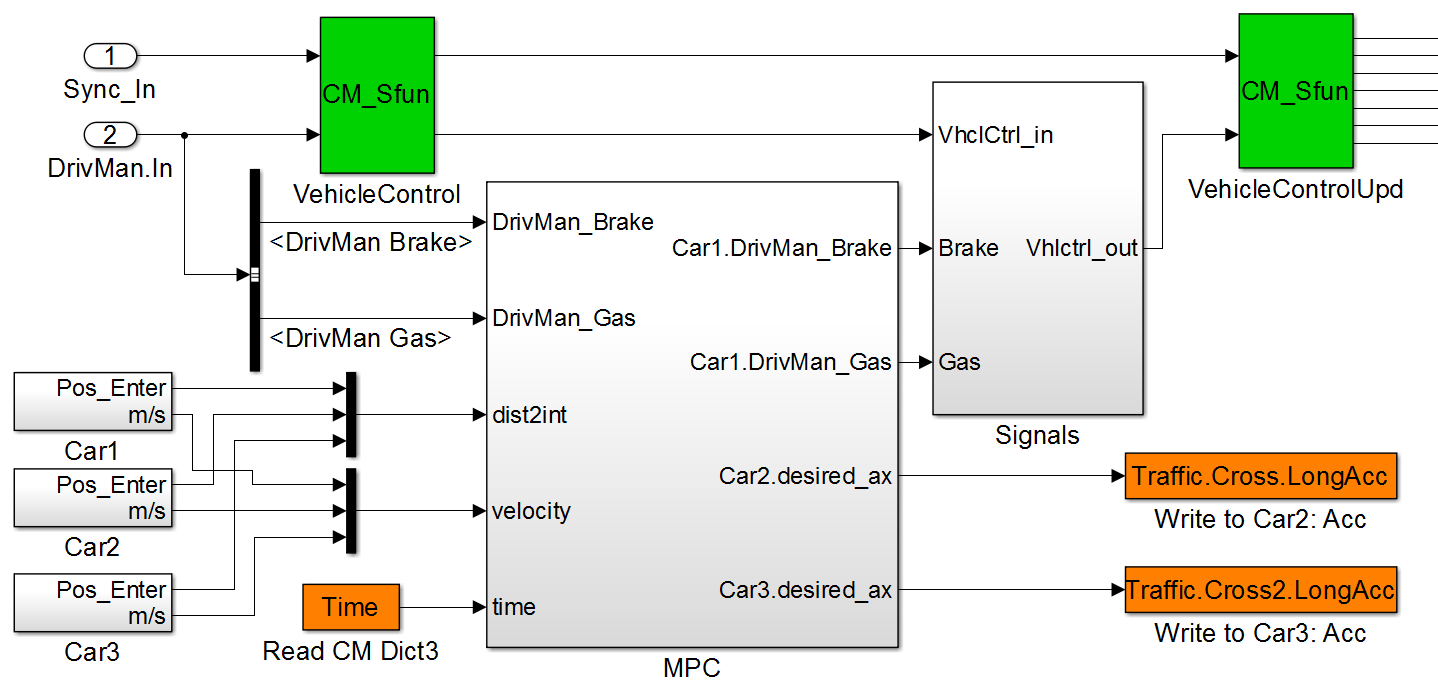
\includegraphics[width=1.8\columnwidth]{CarMaker_Implement2.png}
    \caption{Implementation of the MPC in Simulink combined with CarMaker's Simulink environment.}
    \label{fig:CM_Implement}
\end{figure*}
After implementing the MPC, its performance needs to be validated. Since a simplified point mass model for the vehicle dynamic is used for the controller design, it is reasonable to test the MPC on a more advanced car model.\\ \indent
For the simulation, a combination of Matlab/Simulink and CarMaker is used. In this section, the focus is on connecting the MPC developed in Matlab/Simulink to a traffic model created with CarMaker. The MPC is implemented as a Matlab Function block in Simulink. The simulation tool IPG CarMaker serves as a simulation environment to design a traffic model, containing an intersection and traffic flow, for the case study later described. CarMaker provides more advanced car models. These are used in the simulation to test if collisions are still avoided when the controller is applied to these more detailed vehicle models instead of the point mass models. It is also possible in CarMaker to change the type or only some parameters of a car. Furthermore, CarMaker provides a video animation by the plug in program IPG Movie for visualizing the simulation results. This simplifies the validation of the simulation results.
\subsection{Restrictions of CarMaker}
\subsubsection{CarMaker for Simulink}
The simulation speed for running CarMaker in Simulink is very slow, especially with additional models. Even little add-ons to the generic vehicle model can lead huge loss in performance \cite{qsguide}. Simulations with the MPC Matlab function block included are therefore very time consuming.
\subsubsection{Vehicle models}
A significant drawback of using CarMaker as a simulation environment in this case, is that CarMaker provides only one host car simulated as an advanced car model. It is not possible to control several vehicles with all their vehicle dynamics. Except of the host car, all other cars can only be modeled as traffic objects, which implies static objects without dynamics. They are simulated as 3-D boxes with a certain initial position and acceleration. The acceleration of each traffic object can be overwritten with the output of the MPC, but it should be noted that these cars have similar dynamics as the point mass model used for the controller design.
\subsubsection{Road model}
A CarMaker road is constructed from start to stop by a list of road segments, each one only connected with the previous and following segment \cite{guide}. Thus, it is difficult to construct an intersections, because it is a multiple choice path. For simplicity, an intersection can be constructed by making a turn and letting the road cross itself (see Fig. \ref{fig:CarM}). This causes a limitation to the movements of the vehicles because the motion of the traffic objects is connected to the definition of the road. Thus, the traffic objects have to pass straight through the intersection. A turn in such intersection is not possible.
\subsection{Simulation environment design}
In CarMaker, it is possible to design different test traces with various numbers of intersecting arcs and lanes in the arc. After the realization of a test trace including an intersection, traffic is added to the model. For each vehicle, the host car as well as the traffic objects, the vehicle type, the reference starting point and reference speed are preset.\\
Since the host car starts always with zero velocity, the road model should be designed in a way such that the host car has reached its desired speed before entering the controlled intersection surrounding. 
\subsection{Adding the MPC}
In CarMaker for Simulink, it is possible to change the vehicle model itself. The model generic.mdl given by CarMaker provides a basic CarMaker model without any additional control blocks \cite{qsguide}. It is used as a start-up model to connect the simulation environment created in CarMaker with the MPC Matlab Function block in Simulink. The CarMaker simulation model in Simulink consists of a chain of individual subsystem blocks. These blocks can not be removed, but their functionality can by changed by overwriting their input or output signals.\\ \indent
The model generic.mdl contains the following models as subsystems: \textit{Driver/Driving Maneuver}, \textit{Vehicle Control} and \textit{Vehicle}. To include the MPC block, the subsystem \textit{Vehicle Control} is modified. 
By hijacking the gas and brake signals in the \textit{Vehicle Control} block in Simulink as seen in Fig. \ref{fig:CM_Implement}, the drivers wish is overwritten by the calculated values from the MPC algorithm. The gas and brake signals from the driver model is only used for the vehicle with dynamics, where the control signal calculated by the MPC for this vehicle is converted to the gas and brake signals. For the other vehicles which are static traffic objects, there is no driver model. Therefore, the calculated control signals for these two vehicles overwrite directly the acceleration signal without a conversion to gas and brake signals.
\section{Case study: Controlling three vehicles}
In the selected case study, the presented MPC is tested for three cars approaching an intersection as shown in Fig. \ref{fig:CarM}.
\begin{figure}[h!]
    \centering
    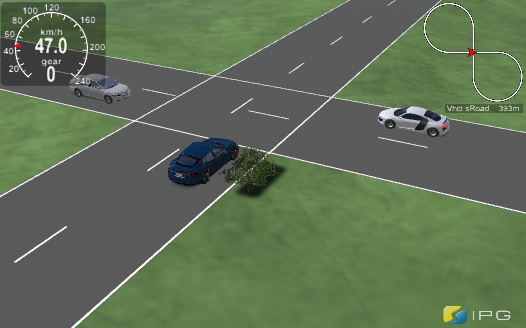
\includegraphics[width=0.9\columnwidth]{Intersection_CarMaker.png}
    \caption{Created intersection crossing in CarMaker environment where the three case are approaching the intersection.}
    \label{fig:CarM}
\end{figure}
%% add picture
%%maybe we have to actualize this table in the end 
% !!!!!
\begin{table}[h!]
\renewcommand{\arraystretch}{1.3}
\caption{Problem data of the case study.}
\label{data}
\centering
\begin{tabular}{c|c}
\hline
\bfseries Parameter & \bfseries Values\\
\hline
$\begin{pmatrix}v_{1r}& v_{2r}& v_{3r}\end{pmatrix}$ & $\begin{pmatrix} \unitfrac[47]{km}{h}& \unitfrac[48]{km}{h}&\unitfrac[50]{km}{h}\end{pmatrix}$\\
$\begin{pmatrix}v_{imin}& v_{imax}\end{pmatrix}$ & $\begin{pmatrix} \unitfrac[30]{km}{h}& \unitfrac[90]{km}{h}\end{pmatrix}$\\
$\begin{pmatrix}a_{imin}& a_{imax}\end{pmatrix}$ & $\begin{pmatrix} \unitfrac[-3]{m}{s^2}& \unitfrac[3]{m}{s^2}\end{pmatrix}$\\
$\begin{pmatrix} w_{i1} &w_{i2} &w_{i3} & w_{i4}\end{pmatrix}$&
$\begin{pmatrix} 1  &  5 & 7 & 1000 \end{pmatrix}$ \\
$\Delta t$ & \unit[0.6]{s}\\
\hline
\end{tabular}
\end{table}
Table \ref{data} contains the chosen parameters for the cars $i=1,2,3$. In this case, the speed and acceleration limits as well as the weights for the cost function are selected identically for all three vehicles. The desired crossing sequence is chosen to $1,2,3$. The vehicles start with different initial speed and distances from the intersection. Without a controller, car $1$ and $2$ would collide in the intersection. The MPC takes control over a vehicle when it has entered the control radius of the intersection, which is $60$ meters before and $60$ meters after the intersection. The critical region, where no collisions are allowed, is the $15\cdot15$ $m^2$ intersection crossing area. For simplicity, the vehicles do not turn left or right in the intersection, instead they only drive straight forward. The initial optimization horizon for every car entering the control area is N=135 meters.\\ \indent 
Gathered data from the sensors of the vehicles via CarMaker is shown in Fig. \ref{fig:sim_results}. When vehicle $1$ is getting closer to the intersection it can be observed that the vehicle starts to accelerate and vehicle $2$ starts decelerating in order to avoid a collision between the two. The third vehicle will also slow down closely after to avoid a collision between the second and third vehicle. One notable part in these figures are the acceleration of the static vehicles without dynamics in the middle plot, i.e. vehicle 2 and vehicle 3. Their acceleration is fluctuating considerably more than vehicle 1 which is the vehicle with dynamics. One explanation is that the acceleration of these two static cars is directly fed from the MPC algorithm, whereas for the first car, it will be converted to gas and brake signals via a PI controller. Additional tuning on the jerk penalty of the static cars in the cost function may decrease the fluctuation. Furthermore, by looking at the last plot, it is evident that the MPC controller prohibits efficiently collisions  between the vehicles. An upward-pointing triangle means the time where the vehicle is entering the intersection and an downward-pointing triangle shows the time when it is leaving. Since there is no vertical alignment between an downward-pointing triangle and an upward-pointing triangle, there are no collisions. CarMaker provides also a video animation for visualizing the simulation results. In the video, it can also be observed that the cars drive in a smooth way following the given crossing sequence and there is never more than one car in the intersection.
\begin{figure}[h!]
    \centering
    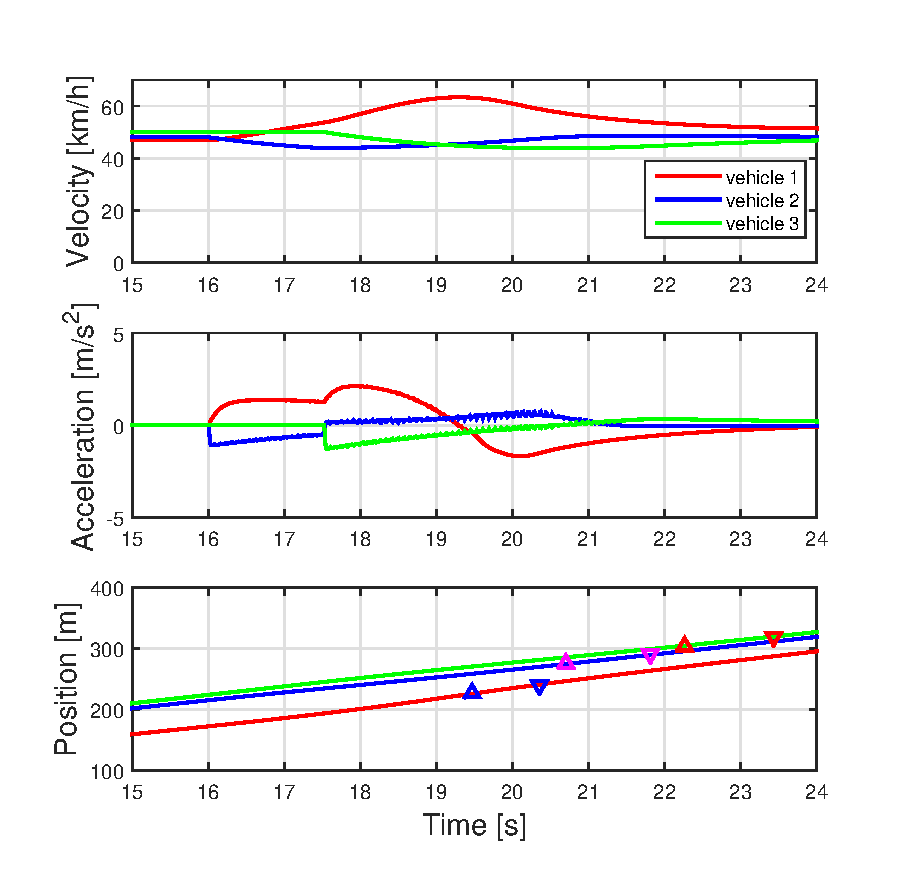
\includegraphics[width=0.52\textwidth]{plots_dpc.eps}
    \caption{Optimal trajectories from the MPC controller. The three subplots show velocity, acceleration and position.}
    \label{fig:sim_results}
\end{figure}
\section{Conclusions}
This paper provides a centralized MPC for optimal control of autonomous vehicles in the control area of an intersection. The problem is formulated as a convex quadratic problem such that the MPC equations can be solved efficiently. The controller is tested for an advanced vehicle model using the simulation tool CarMaker. Simulation results are shown in a case study showing that the MPC works efficiently for the advanced CarMaker vehicle model.\\ \indent
Compared to the solution presented in \cite{nikolce}, the computation time for the convex problem is decreased by using a QP solver instead of the generalized second order cone program (SOCP) solver. Using the quadratic form for the MPC, the problem can be solved very fast in every time step. The computation time is related to the distance to the intersection of each vehicle. Since it depends on the number of cars in the control area and the length of their prediction horizon, the computation time is decreased by using a shrinking prediction horizon.\\ \indent
In the MPC design, the vehicle dynamic is modeled as a simplified point mass model. Testing the controller for an advanced vehicle model by combining CarMaker and Matlab/Simulink shows that all constraints are fulfilled, especially the prohibition of collisions. The MPC works efficiently for the virtual test drive, but using CarMaker as a simulation environment turned out to have some significant drawbacks. CarMaker provides an advanced vehicle model only for the host car. Thus, it is more realistic than using only point masses for the simulation, but since the other cars are static objects, it is questionable if it is suitable as a reliable test platform for an intersection crossing problem like this. Furthermore, due to the immense computation time for simulations, where the simulation environment of CarMaker is combined with the MPC in Matlab/Simulink, it is very costly to test the MPC for the presented simple case study. Thus, testing the virtual test drive with changed parameters like adjusted weights is problematic because of the expenditure of time. For a more extended case study, e.g. with more cars in the control area, CarMaker combined with Matlab/Simulink can be considered as ineffective as a virtual test basis.\\ \indent
Though CarMaker may be not the best choice as a simulation tool in order to validate the control algorithm, the program was useful to visualize and validate the controller output in a 3d environment with the plug in program IPG Movie. After a simulation it is possible to view a video animation in several different angles and camera positions and also export the visualization as movies or photos as in Figure \ref{fig:CarM}.\\ \indent
In this paper, a fixed crossing sequence is used for testing the MPC due to the restrictions in computation time using CarMaker. The optimal crossing sequence could be found by computing the optimal solution for all permutations of crossing sequences and selecting the crossing sequence that minimizes the cost function as described in \cite{nikolce}. For applying that and validating the efficiency of the presented controller in more extended virtual case studies with more cars, desirable all with an advanced vehicle model, another simulation environment needs to be found or the existing code has to be improved regarding computation speed. A simulation environment, that can be combined with Matlab/Simulink and may be more efficient in this case, is the simulation tool PreScan, but further research on this has to be done. Future work may focus on testing other simulation strategies to validate the controller in extended virtual case studies. Another research branch may be the extension of the formulated convex problem focusing on other objectives and constraints, e.g. safety constraints when several vehicles travel on the same path. 

%Another subject to investigate further is the need of adding an extra constraint for the collision avoidance. The MPC algorithm uses the current longitudinal position of each vehicle as a index of the distance to the intersection. One drawback and problem occurs when a vehicle is entering the critical region. The index of when the vehicle entered the critical zone will then be a negative integer, which can't be used to describe a index. In the algorithm is the collision avoidance constraint hence only activated until the second vehicle enters the critical region. This constraint fulfills the criteria avoid collision in this case study but a more detailed constraint that can handle negative distance to the intersection can be a more generalized solution. For example if a second vehicle $c2$ entered the intersection one meter ago, then the first car $c1$ have to be 1 meter past the critical region. 

%Also, by using position as index variable for the control algorithm restrict the step index to be a at least one meter. The actual position in the Simulation environment is not all ways fulfilling this criteria and therefore is the current longitudinal position needed to be rounded to a integer value.


%\section{to do}
%\begin{itemize}
%\item matrices from result chapter generalized in the mpc chapter
%\item modeled in space, simulated in time --> position input mpc, rounding
%\item we write in the case study about how the system is able to avoid collisions efficiently, but in the introduction we mention that this system would be able to decrease fuel consumption. In the cost function you also mention that the system should penalize longitudinal acceleration and jerk to guarantee a comfortable drive. Do you have any results regarding these issues? That the system actual will decrease fuel consumption and give a comfortable drive? --> write something 
%\item conclusions:how could it be implemented on real cars. kind of supervision that controls the incoming cars?
%\item You mention that the MPC can solve the problem very fast in every step. How fast is this? Is it fast enough to run in realtime on a car?
%\end{itemize}
\bibliographystyle{IEEEtran}
\bibliography{database}

\end{document}
